\chapter{Background}
\label{sec:background}

\section{Bunge-Wand-Weber ontology}

A \textbf{conceptualization} is an abstract, simplified view of the world that is represented for
some purpose~\cite{gruber1995toward}. It consists of the concepts that are assumed to exist in some
area of interest and their relationships~\cite{gruber1995toward}. An \textbf{ontology} is an
explicit specification of a conceptualization~\cite{gruber1995toward}. It describes what is
fundamental in the totality of what exists and it defines the most general categories to which we
need to refer in constructing a description of reality~\cite{milton2004top}.

Researchers distinguish between two kinds of ontologies: top-level and domain-
specific~\cite{milton2004top}. Ontologies of the former type are highly general and provide the
theoretical foundations for representation and modeling of systems. Ontologies of the latter type
define concepts and their relations only for a particular domain. A domain- specific ontology is
based on a specific top-level ontology if it uses the categories defined by the high level
ontology~\cite{milton2004top}.

The Bunge-Wand-Weber (BWW) ontology~\cite{wand1990ontological} is a high-level ontology used in the
representation model developed by Wand and Weber~\cite{wand1995deep}. Table \ref{tab:bwwmodel}
presents a selected set of the ontological constructs in the BWW ontology.

\begin{center}
\begin{longtable}{ | p{11em} | p{30em} | } 
\caption{Selected ontological constructs in the BWW representation model}
\label{tab:bwwmodel}\\
\hline
 &  \\
\textbf{Ontological construct} & \textbf{Explanation} \\
 &  \\
\hline
Thing & The elementary unit in the BWW ontological model. The real world is made up of things. A composite thing may be made up of other things (composite or primitive).~\cite{wand1995deep} \\ 
\hline
Properties & \multirow{7}{30em}{Things possess properties. A property is modeled via a function that maps the thing into some value. A property of a composite thing that belongs to a component thing is called an hereditary property. Otherwise it is called an emergent property. A property that is inherently a property of an individual thing is called an intrinsic property. A property that is meaningful only in the context of two or mode things is called a mutual or relational property.~\cite{wand1995deep}} \\ 
 &  \\ 
 &  \\
 &  \\
 &  \\
 &  \\
 &  \\
 \hline
 State & A vector of values for all property functions of a thing.~\cite{wand1995deep} \\
 \hline
 Event & A change of state of a thing. It is effected via a transformation.~\cite{wand1995deep} \\
 \hline
 Transformation & A mapping from a domain comprising states to a codomain comprising states.~\cite{wand1995deep} \\
 \hline
 History & The chronologically ordered states that a thing traverses.~\cite{weber1996analytical} \\
 \hline
 Coupling & A thing acts on another thing if its existence affects the history of the other thing. The two things are said to be coupled or interact.~\cite{wand1995deep} \\
 \hline
 Class & A class is a set of things that can be defined via their possessing a characteristic property.~\cite{weber1996analytical} \\ 
 \hline
 Subclass & A set of things that can be defined via their possessing the set of properties in
a class plus an additional set of properties.~\cite{weber1996analytical} \\ 
\hline
 System & A set of things is a system if, for any bi-partitioning of the set, couplings exist among things in the two subsets.~\cite{wand1995deep} \\
 \hline
 System Composition & The things in the system are its composition.~\cite{wand1995deep} \\
 \hline
 System Environment &  Things that are not in the system but interact with things in the system are called the environment of the system.~\cite{wand1995deep} \\
 \hline
\end{longtable}
\end{center}


\section{Ontological analysis}

\textbf{Ontological analysis} is an established approach for evaluating the quality of software engineering notations~\cite{moody2009physics}. It consists of a two way comparison between a set of modeling grammar constructs and a set of ontological constructs. The \textbf{interpretation mapping} compares the notation with the ontology and the \textbf{representation mapping} compares the ontology with the notation~\cite{gehlert2007toward}. The underpinning of ontological analysis is that modeling grammars are incomplete if they are not able to represent what exists in reality~\cite{green2000integrated}. Furthermore, the analysis requires one-to-one mapping between the modeling grammar and the ontological constructs. Any deviation from such correspondence leads to a discrepancy (Figure \ref{fig:ontoanalysis}).

\begin{figure}[h!]
  \centering
  \caption{Ontological Analysis~\cite{gehlert2007toward}}
  \label{fig:ontoanalysis}
  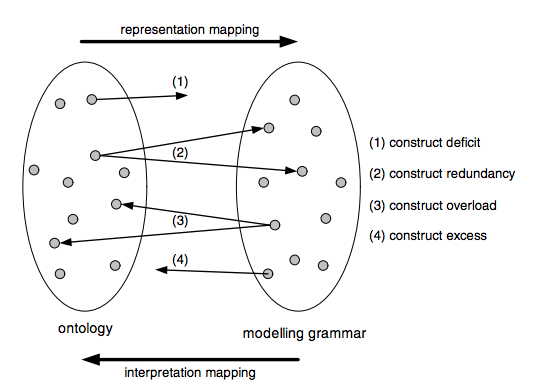
\includegraphics[width=0.65\textwidth]{ontoanalysis}
\end{figure}

\textbf{Construct deficit} occurs when an ontological construct does not have a corresponding construct in the modeling grammar. \textbf{Construct redundancy} is observed when a single ontological construct maps to more than one modeling grammar construct. \textbf{Construct overload} appears when a modeling grammar construct corresponds to more than one ontological construct. \textbf{Construct excess} emerges when a modeling grammar construct does not map to any ontological construct.~\cite{moody2009physics}

